\documentclass[11pt]{article}
\usepackage[margin=1in]{geometry}
\usepackage{graphicx}
\usepackage{booktabs}
\usepackage{amsmath}
\usepackage{hyperref}
\usepackage{xcolor}

% Auto-generated macros -- every number in this document should come from
% here, not be hand-typed. Regenerate with: python paper/extract_numbers.py
% AUTO-GENERATED by paper/extract_numbers.py -- do not hand-edit.
% Every number here traces to a specific reports/**/*.json file; rerun
% the extraction script (not this file) if an upstream number changes.

\newcommand{\AucKlGaussianOneThreeM}{7.95}
\newcommand{\AucKlGaussianThreeSevenM}{3.80}
\newcommand{\AucKlOnManifoldOneThreeM}{3.32}
\newcommand{\AucKlOnManifoldThreeSevenM}{2.07}
\newcommand{\AucKlPermutedOneThreeM}{23.47}
\newcommand{\AucKlPermutedThreeSevenM}{2.80}
\newcommand{\AucKlRelatedOneThreeM}{1.47}
\newcommand{\AucKlRelatedThreeSevenM}{0.81}
\newcommand{\AucKlSameContextOneThreeM}{0.00}
\newcommand{\AucKlSameContextThreeSevenM}{0.00}
\newcommand{\AucKlUnrelatedOneThreeM}{2.42}
\newcommand{\AucKlUnrelatedThreeSevenM}{1.55}
\newcommand{\DepthTrendTop1OneThreeM}{-0.392}
\newcommand{\DepthTrendTop1ThreeSevenM}{-0.569}
\newcommand{\EchoRatePctOneThreeM}{19.8\%}
\newcommand{\EchoRatePctThreeSevenM}{19.8\%}
\newcommand{\EchoRetainedPctOneThreeM}{86\%}
\newcommand{\EchoRetainedPctThreeSevenM}{85\%}
\newcommand{\GaussianMinusOnManifoldOneThreeM}{4.62}
\newcommand{\GaussianMinusOnManifoldThreeSevenM}{1.73}
\newcommand{\LeveragePearsonOneThreeM}{-0.083}
\newcommand{\LeveragePearsonThreeSevenM}{0.009}
\newcommand{\NContextsOneThreeM}{1200}
\newcommand{\NContextsThreeSevenM}{1200}
\newcommand{\NLayersAboveFloorOneThreeM}{21/24}
\newcommand{\NLayersAboveFloorThreeSevenM}{40/48}
\newcommand{\NLayersFullAboveFloorOneThreeM}{23/24}
\newcommand{\NLayersFullAboveFloorThreeSevenM}{47/48}
\newcommand{\NLayersNonEchoAboveFloorOneThreeM}{22/24}
\newcommand{\NLayersNonEchoAboveFloorThreeSevenM}{42/48}
\newcommand{\NRecentK}{3}
\newcommand{\OnManifoldMinusUnrelatedOneThreeM}{0.90}
\newcommand{\OnManifoldMinusUnrelatedThreeSevenM}{0.51}
\newcommand{\ParticipationRatioMaxOneThreeM}{1.09\%}
\newcommand{\ParticipationRatioMaxThreeSevenM}{0.70\%}
\newcommand{\ParticipationRatioMinOneThreeM}{0.019\%}
\newcommand{\ParticipationRatioMinThreeSevenM}{0.012\%}
\newcommand{\PeakLayerOneThreeM}{3}
\newcommand{\PeakLayerThreeSevenM}{3}
\newcommand{\PearsonROneThreeM}{-0.532}
\newcommand{\PearsonRThreeSevenM}{-0.613}
\newcommand{\ShapeShareOneThreeM}{83.6\%}
\newcommand{\ShapeShareThreeSevenM}{77.2\%}
\newcommand{\SpearmanROneThreeM}{-0.734}
\newcommand{\SpearmanRThreeSevenM}{-0.746}


% Visible marker for anything the agent scaffolded structurally but did
% not write the interpretive content for. Search-and-destroy before
% submission; every instance is something Jay writes.
\newcommand{\todojay}[1]{\textcolor{red}{\textbf{TODO(jay):} #1}}

\title{Closed-Loop Architectural Proprioception in Pretrained \\ State-Space Models}
\author{Jay Noon}
\date{\today}

\begin{document}
\maketitle

\begin{abstract}
\todojay{Abstract. Should state: (1) the question -- does a
vocabulary-anchored introspective workspace, found in transformers,
exist in pretrained SSMs, and does it extend to the object that persists
across time; (2) the Gate G1 answer (protocol \S4.4, decided
2026-07-08, \texttt{protocol/GATE\_G1\_DECISION.md}) -- no, not in the
same form: the readable signal is pervasive and early-peaking
(\BandWidthPctOneThreeM/\BandWidthPctThreeSevenM\ of depth, peak layer
\PeakLayerOneThreeM) rather than banded and mid-network
(\BandWidthPctPyFourTen\ in Pythia), and the persistent state is
causally real but mostly generic manifold membership, thinly content --
scoped explicitly to the representational signature, not a claim about
functional/causal workspace existence; (3) the headline quantitative
results: thin saturating legibility signal, disruption law
$d = k(1-\mathrm{sim})$, shape/content decomposition
(\ShapeShareOneThreeM/\ShapeShareThreeSevenM\ of transplant disruption
is generic manifold membership, not content), participation ratio
\ParticipationRatioMinOneThreeM--\ParticipationRatioMaxOneThreeM\ of
ambient dimension; (4) reproducibility claim -- entire study runs on a
4GB consumer laptop GPU.}
\end{abstract}

\section{Introduction}
\todojay{Motivate from protocol/gamma\_protocol.md \S1: Project Beta's
recurrent-state anticipation result + Anthropic's transformer workspace
result, composed. State the G1a/G1b split (Amendment 2) as the paper's
organizing move -- stream vs. genuine state are different objects with
different answers, and that dissociation is itself the finding, not a
methodological footnote.}

\section{Background}
\todojay{Related work stubs -- fill in citations:}
\begin{itemize}
  \item \todojay{Anthropic, \emph{Emergent Introspective Workspace} (transformer-circuits.pub, 2026) -- the motivating transformer result.}
  \item \todojay{Logit lens (nostalgebraist) and tuned lens (Belrose et al. 2023) -- V1/V2 readout methodology.}
  \item \todojay{Mamba / SSM architecture background (Gu \& Dao) -- $d_\mathrm{inner} \times d_\mathrm{state}$ recurrent state, selective scan.}
  \item \todojay{Activation/outlier-channel literature in transformer quantization -- relevant framing for \S\ref{sec:critical-channel}'s null result, cited as context only (Task 1 of the closing pass did not validate a critical-channel effect, so this is discussed as a considered-and-ruled-out alternative, not a confirmed parallel).}
\end{itemize}

\section{Methods}
\subsection{Checkpoint matrix and hardware}
\todojay{Mamba-130M/370M primary, Pythia-160M/410M comparators (matched
Pile pretraining). RTX 3050, 4GB VRAM -- state the deviation from the
protocol's 12GB baseline explicitly (Amendment 1) and the accessibility
framing this enables.}

\subsection{State extraction: stream vs.\ genuine state}
\todojay{\texttt{StreamExtractor} (residual $x$, mixer output) vs.\
\texttt{RecurrentStateExtractor} (genuine \texttt{recurrent\_states} via
cached step-by-step decoding). Amendment 2's correction: what was
originally called $h_t^{(l)}$ was the mixer's per-token output, not the
persistent state.}

\subsection{Gamma-lens: V1 (zero-shot) and V2 (tuned)}
\todojay{Formula, training procedure (KL-to-final-logits loss,
identity-initialized residual affine for V2 on hidden-size-shaped
streams; low-rank readout \texttt{GammaLensV2State} for the
dimensionality-mismatched genuine state).}

\subsection{Calibration floors}
\todojay{Shuffled-target and Gaussian-matched controls
(\texttt{gamma/controls.py}) -- why a trained affine can manufacture
apparent decodability, and how these floors rule that out.}

\subsection{Transplant harness and the six conditions}
\todojay{\texttt{gamma/patching.py}: \texttt{get\_state\_snapshot},
\texttt{greedy\_continue}, \texttt{teacher\_force\_continue},
\texttt{permute\_snapshot}, \texttt{gaussian\_snapshot\_like},
\texttt{sample\_on\_manifold\_noise}. Six conditions: same-context,
related-context, unrelated-context, permuted-real, Gaussian,
on-manifold noise. Metrics: KL(baseline $\Vert$ transplanted), NLL of
baseline's own greedy continuation under the transplanted state.}

\section{Results}

\subsection{Cross-architecture depth-axis mapping (corrected)}
\label{sec:depth-axis}
\todojay{Figure: \texttt{depth\_axis\_corrected.png} for both Mamba
sizes, alongside Pythia's. State the object-mismatch erratum plainly:
original comparison used Mamba mixer-output vs.\ Pythia residual stream
(different objects); corrected residual-vs-residual comparison shows
Mamba's V2 lens converging at the final layer (KL$\to$0, top1$\to$0.87--0.97)
matching Pythia's pattern.}
\begin{figure}[h]
  \centering
  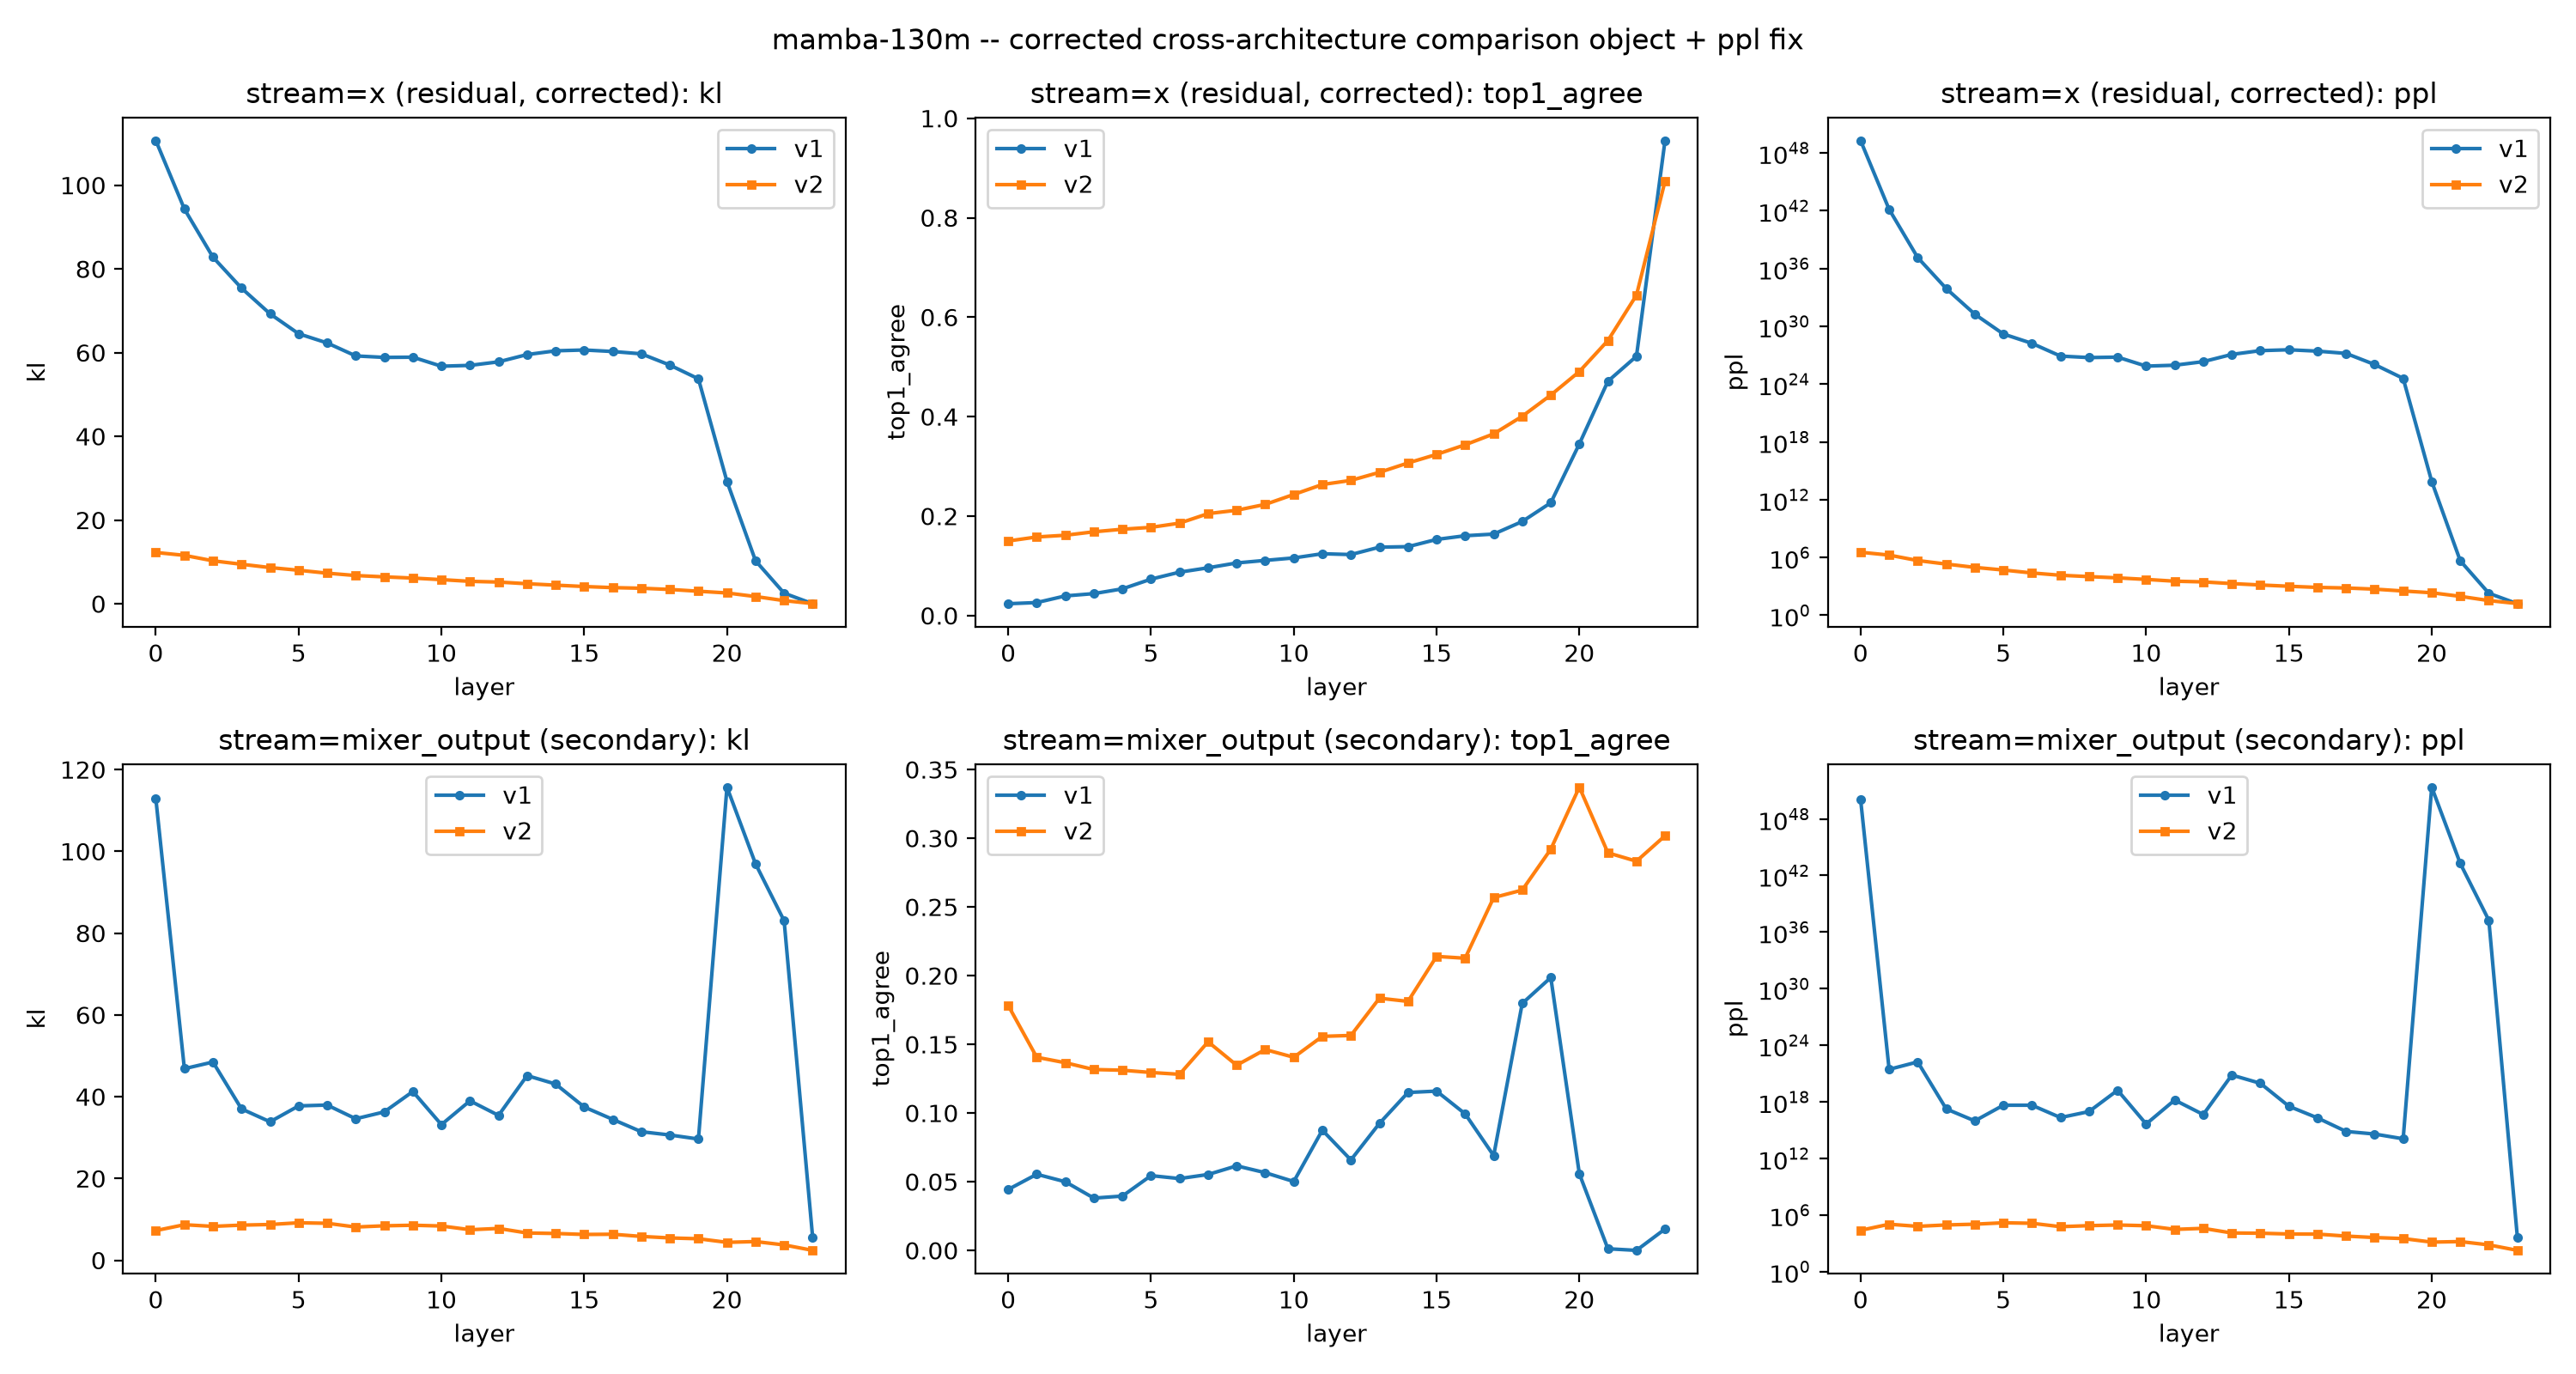
\includegraphics[width=0.48\textwidth]{figures/mamba-130m_depth_axis_corrected.png}
  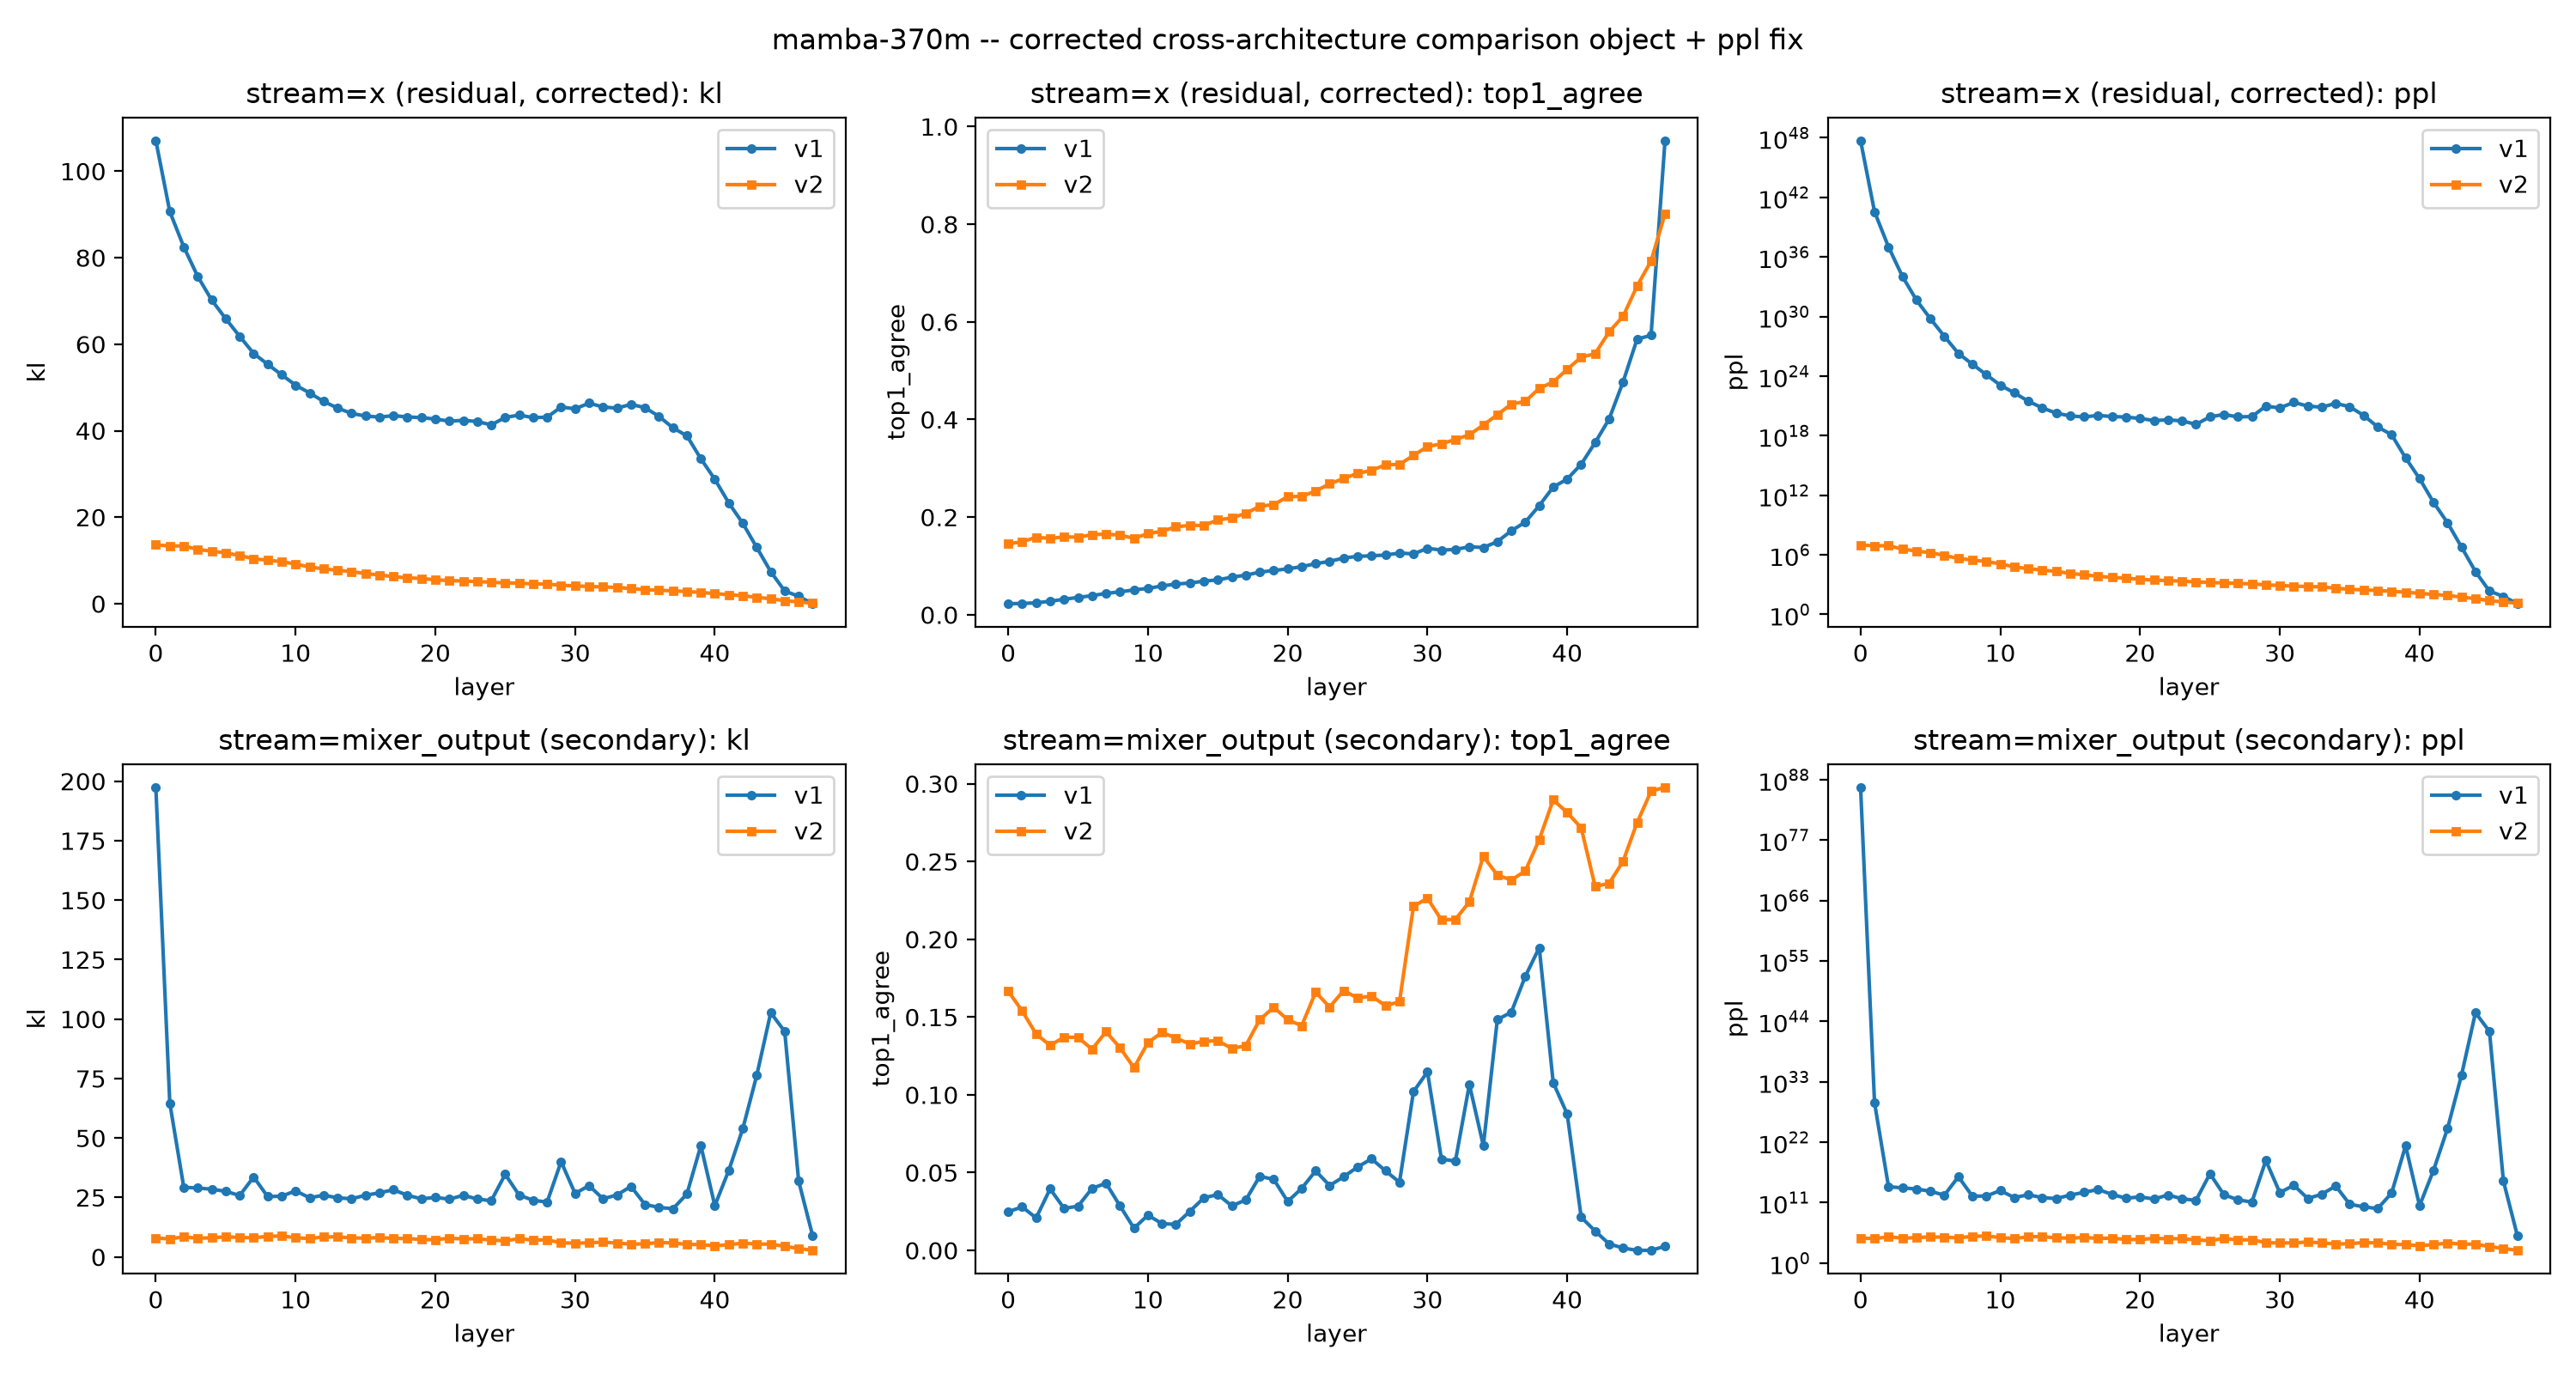
\includegraphics[width=0.48\textwidth]{figures/mamba-370m_depth_axis_corrected.png}
  \caption{\todojay{Caption: corrected residual-stream depth-axis comparison, both Mamba sizes.}}
\end{figure}

\todojay{\textbf{Band width, quantified} (protocol section 4.1.1--2's
input-echo/output-prediction/neither decomposition, applied to the
stream -- reused the already-trained corrected lenses, no retraining).
Band width: Mamba-130M \BandWidthPctOneThreeM\ of depth
(\BandWidthLayersOneThreeM), Mamba-370M \BandWidthPctThreeSevenM\
(\BandWidthLayersThreeSevenM), Pythia-410M \BandWidthPctPyFourTen\
(\BandWidthLayersPyFourTen). State the cross-architecture comparison
plainly: both Mamba sizes show a *wider* band than Pythia-410M at
matched-ish scale, and note this is reported as the pattern found, not
further interpreted (could be architectural, could be V2-calibration
difference). Pythia-160M's \BandWidthPctPyOneSixty\ figure is a ceiling
effect from weak lens convergence at that size (final-layer top1\_agree
only 0.399), not a genuinely wider band -- flag this caveat explicitly,
do not present the four numbers as uniformly comparable. Echo stays
flat and low (5-9\%) at every layer, every model -- the stream is never
mostly copying recent context. See
\texttt{reports/phase1/band\_width.md} for the methodology correction
made before trusting this (an initial version compared against
ground-truth continuation text rather than the model's own future
prediction, and was caught by a sanity check before being reported).}
\begin{figure}[h]
  \centering
  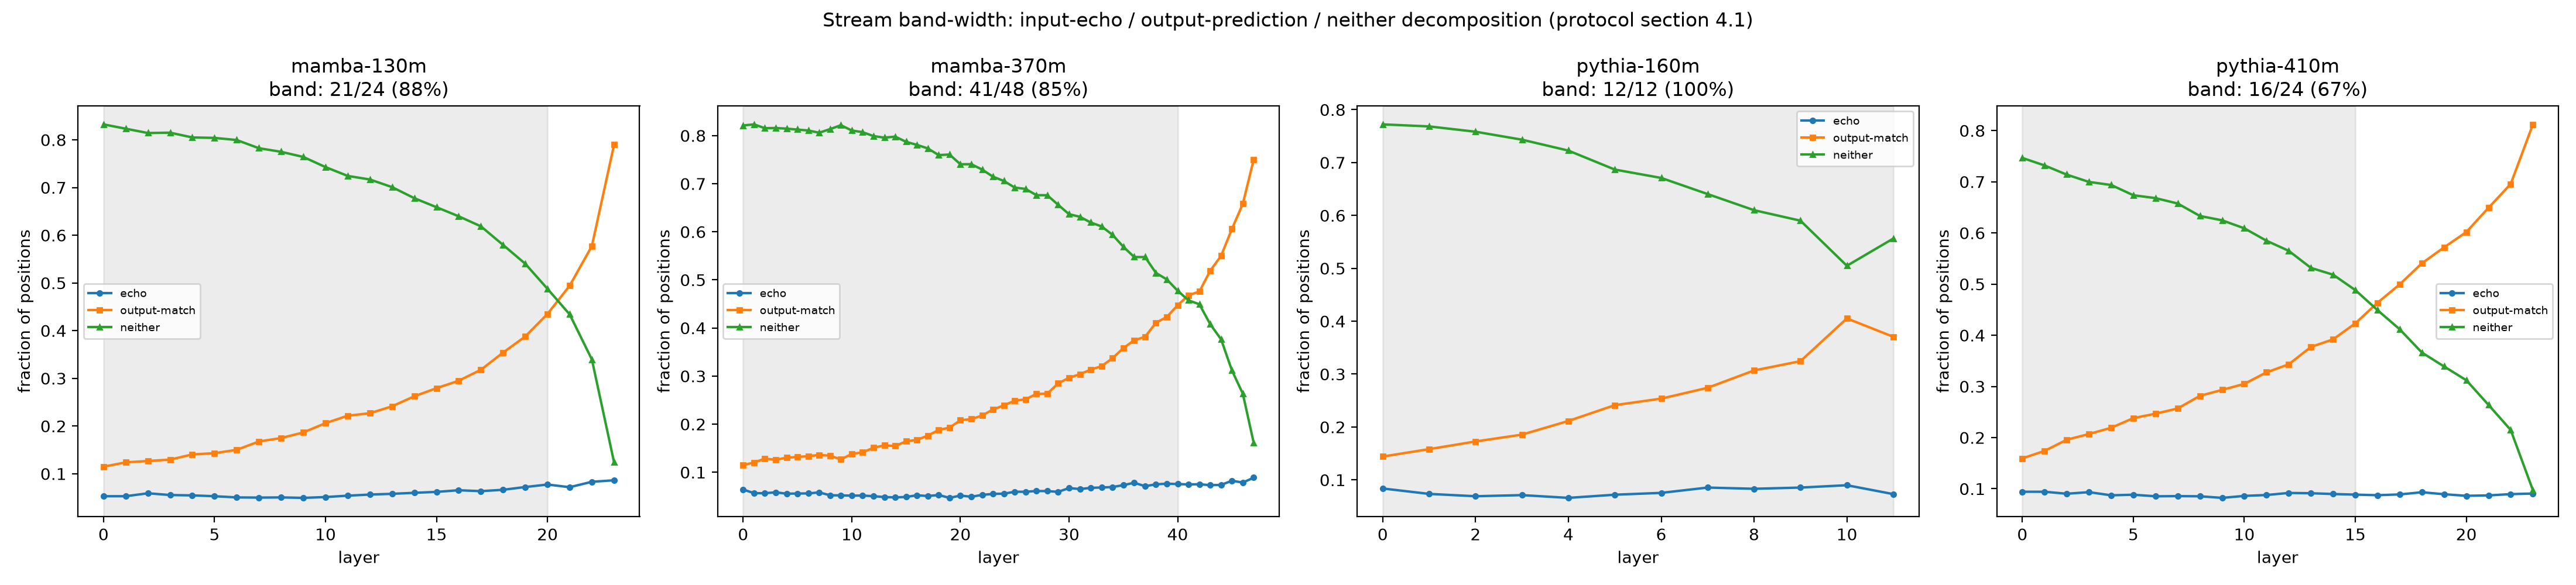
\includegraphics[width=0.95\textwidth]{figures/band_width_plot.png}
  \caption{\todojay{Caption: echo/output-prediction/neither fractions by layer, all four models, band shaded.}}
\end{figure}

\subsection{State legibility: thin, pervasive, and early-peaking, not depth-localized}
\label{sec:legibility}
\todojay{P-A4-4 (depth-localization of the state's argmax-legible
signal) is \textbf{falsified at full scale, both models} --
$N=800$ train / $400$ eval, all layers, both Mamba sizes
(\texttt{scripts/state\_legibility\_depth\_full.py}). Signal is
pervasive (\NLayersAboveFloorOneThreeM\ layers CI-supported at
Mamba-130M, \NLayersAboveFloorThreeSevenM\ at Mamba-370M -- 87.5\% and
83.3\% of all layers respectively), the depth trend is
\emph{negative} at both sizes (Spearman \DepthTrendTop1OneThreeM\ /
\DepthTrendTop1ThreeSevenM, opposite the sign P-A4-4 required), and the
peak is layer \PeakLayerOneThreeM\ of 24 and layer \PeakLayerThreeSevenM\
of 48 respectively -- the same absolute layer index in both models
despite a 2$\times$ depth difference, itself worth a sentence. State
plainly that this directly falsifies the Amendment 4 margin note's
``state channel = stream's workspace band, lower bandwidth'' reading --
not as a band, at least. See \texttt{reports/phase1/state\_legibility\_depth\_full.md}.}
\begin{figure}[h]
  \centering
  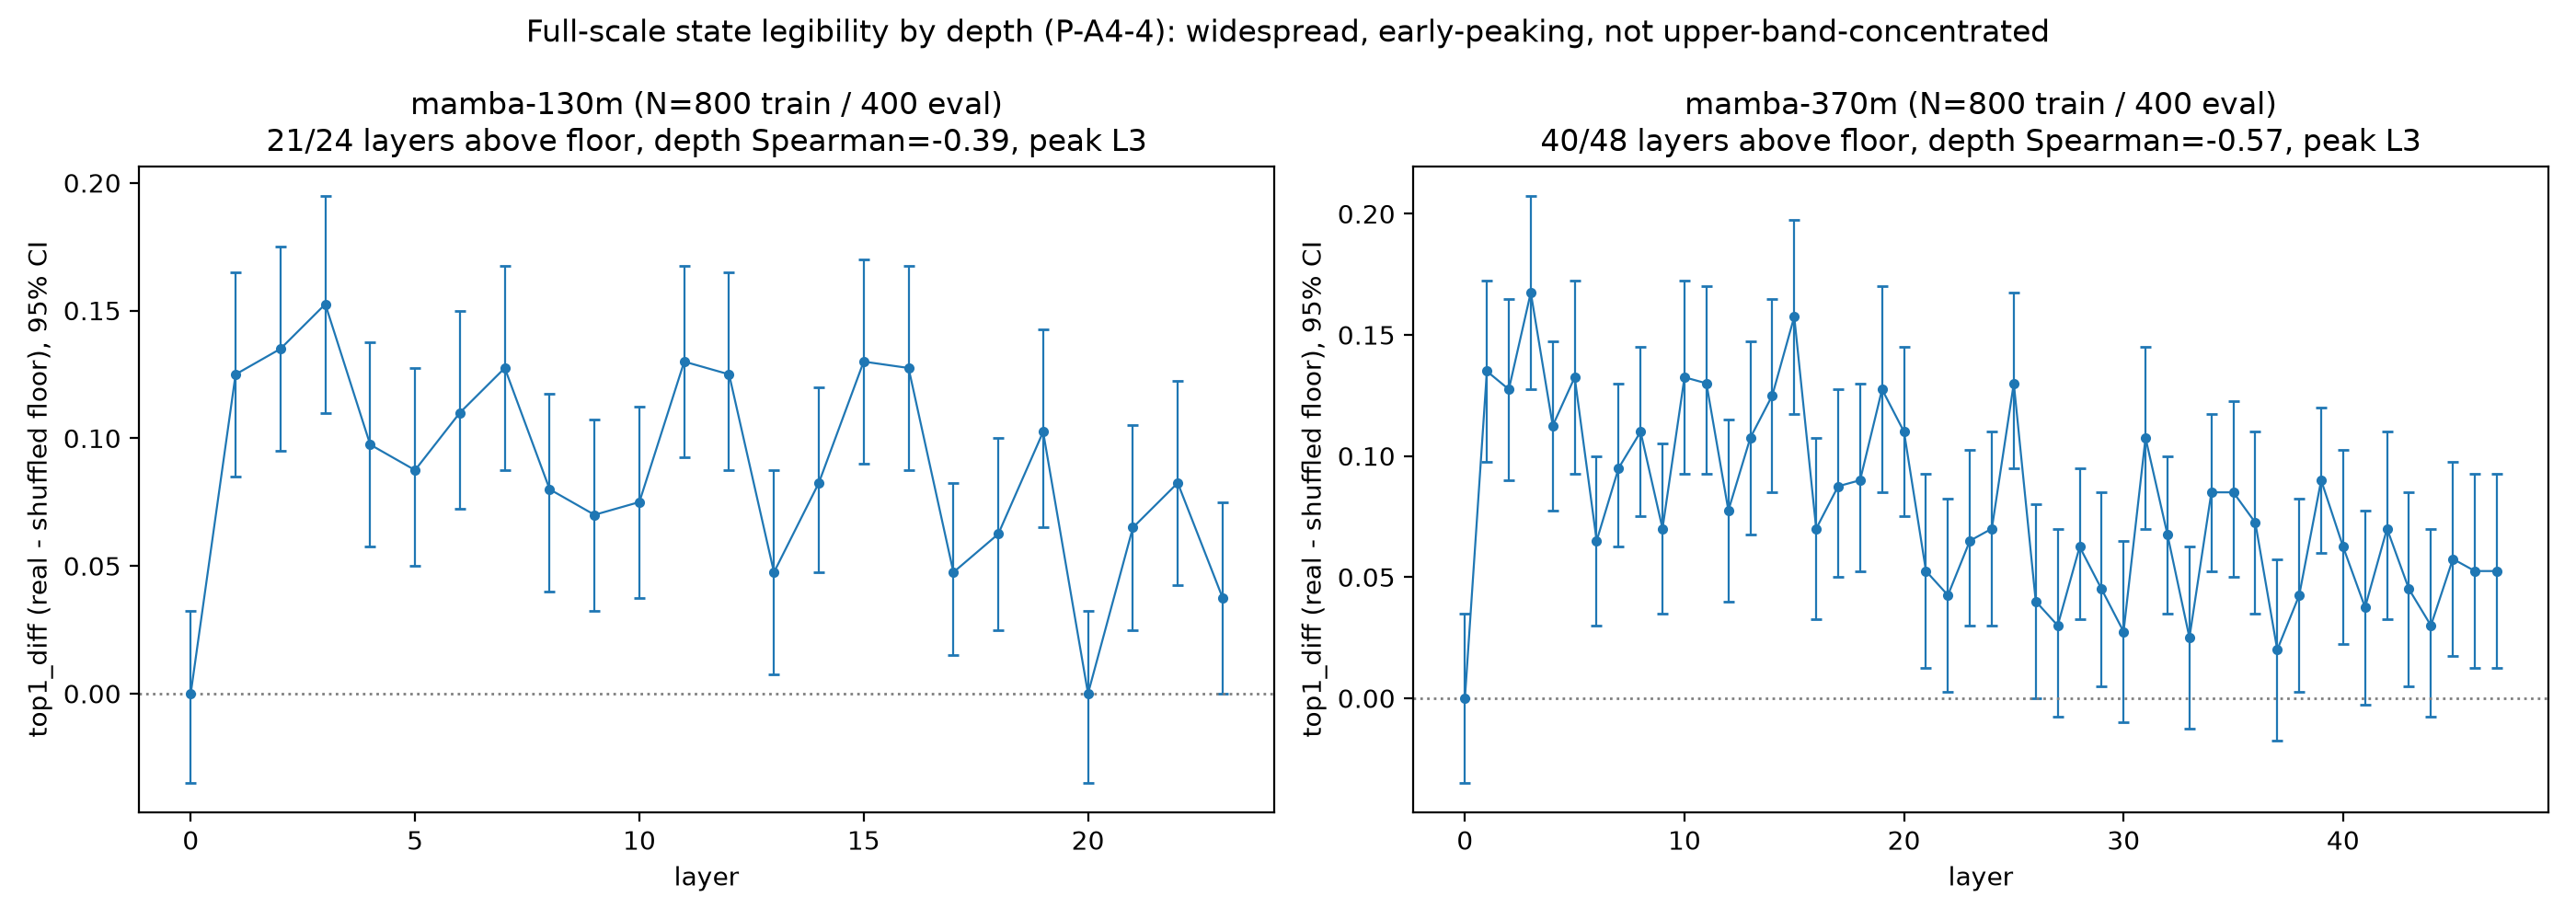
\includegraphics[width=0.95\textwidth]{figures/state_legibility_depth_full.png}
  \caption{\todojay{Caption: full-depth top1-above-floor signal, both models, 95\% CI per layer. Note layer-0 degeneracy (both models exactly zero) and the early-peak/gradual-decline shape.}}
\end{figure}

\todojay{\textbf{Echo-partialling check} (rules out the cheapest
alternative explanation for the above): is the early-peaked signal just
input echo (target token already present in the 16-token prefix)?
Echo rate \EchoRatePctOneThreeM\ of eval examples (any-of-prefix
definition), both models. Excluding echo-explainable examples:
\NLayersNonEchoAboveFloorOneThreeM\ layers still CI-supported at
Mamba-130M (down from \NLayersFullAboveFloorOneThreeM),
\NLayersNonEchoAboveFloorThreeSevenM\ at Mamba-370M (down from
\NLayersFullAboveFloorThreeSevenM) -- signal magnitude retained:
\EchoRetainedPctOneThreeM\ / \EchoRetainedPctThreeSevenM. State the
one-line result plainly: the legible slice is largely distinct from
input echo, not primarily explained by it, at both sizes. See
\texttt{reports/phase1/echo\_partialling.md} for the recent-\NRecentK\
stricter definition (near-identical result) and the scope caveat (exact
token-match echo only, not fuzzy/n-gram echo).}
\begin{figure}[h]
  \centering
  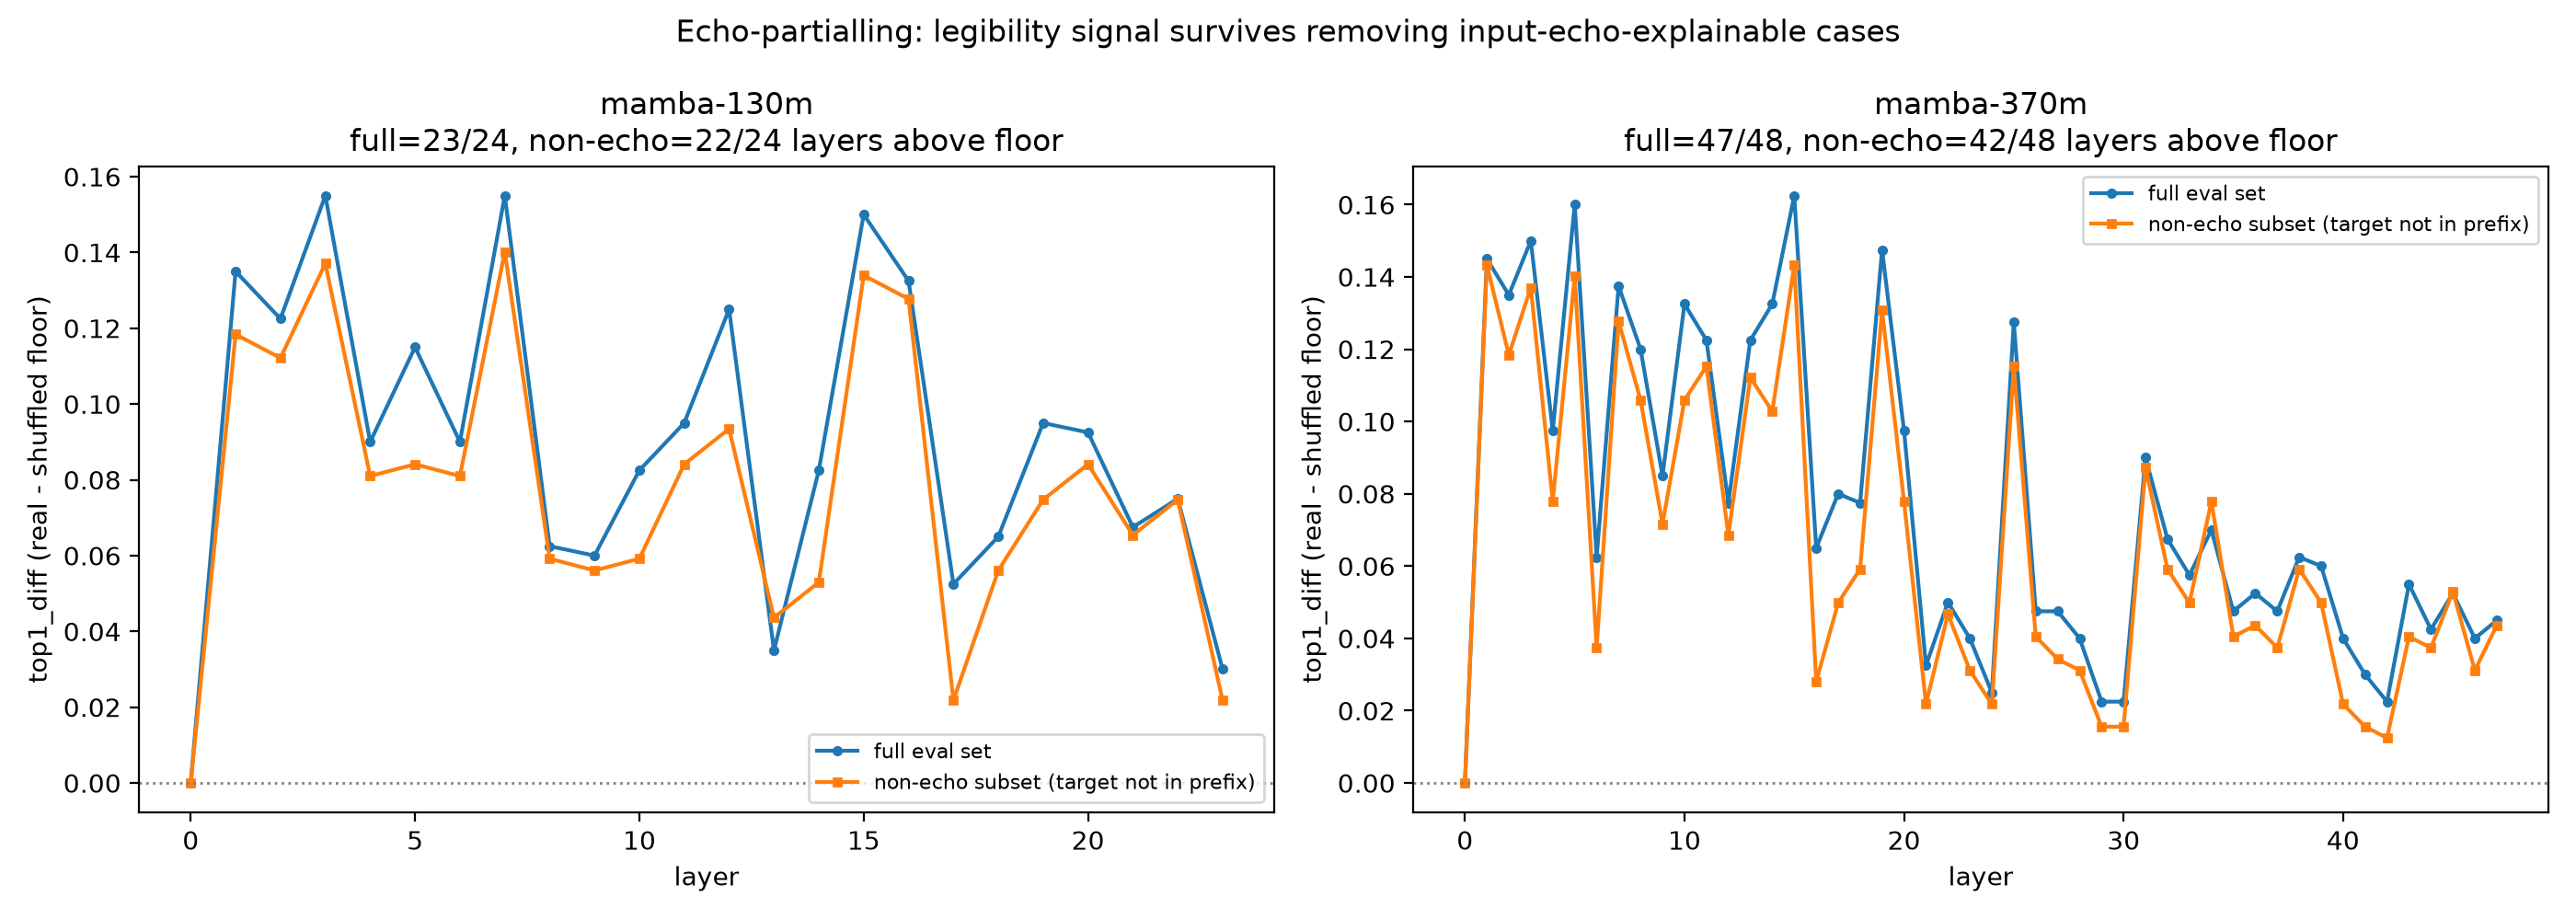
\includegraphics[width=0.95\textwidth]{figures/echo_partialling_plot.png}
  \caption{\todojay{Caption: full eval set vs.\ non-echo subset, per-layer top1-above-floor, both models. Curves track closely at nearly every layer.}}
\end{figure}

\subsection{Manifold geometry: low dimensionality and terminal funneling}
\label{sec:manifold}
\todojay{Participation ratio \ParticipationRatioMinOneThreeM--\ParticipationRatioMaxOneThreeM\
of ambient dimension (Mamba-130M, $N=\NContextsOneThreeM$ held-out
contexts), \ParticipationRatioMinThreeSevenM--\ParticipationRatioMaxThreeSevenM\
(Mamba-370M). State the depth trend: dimensionality collapses sharply
in the final few layers of both models (``terminal funneling'') --
this is a real, reportable structural finding independent of anything
downstream.}
\begin{figure}[h]
  \centering
  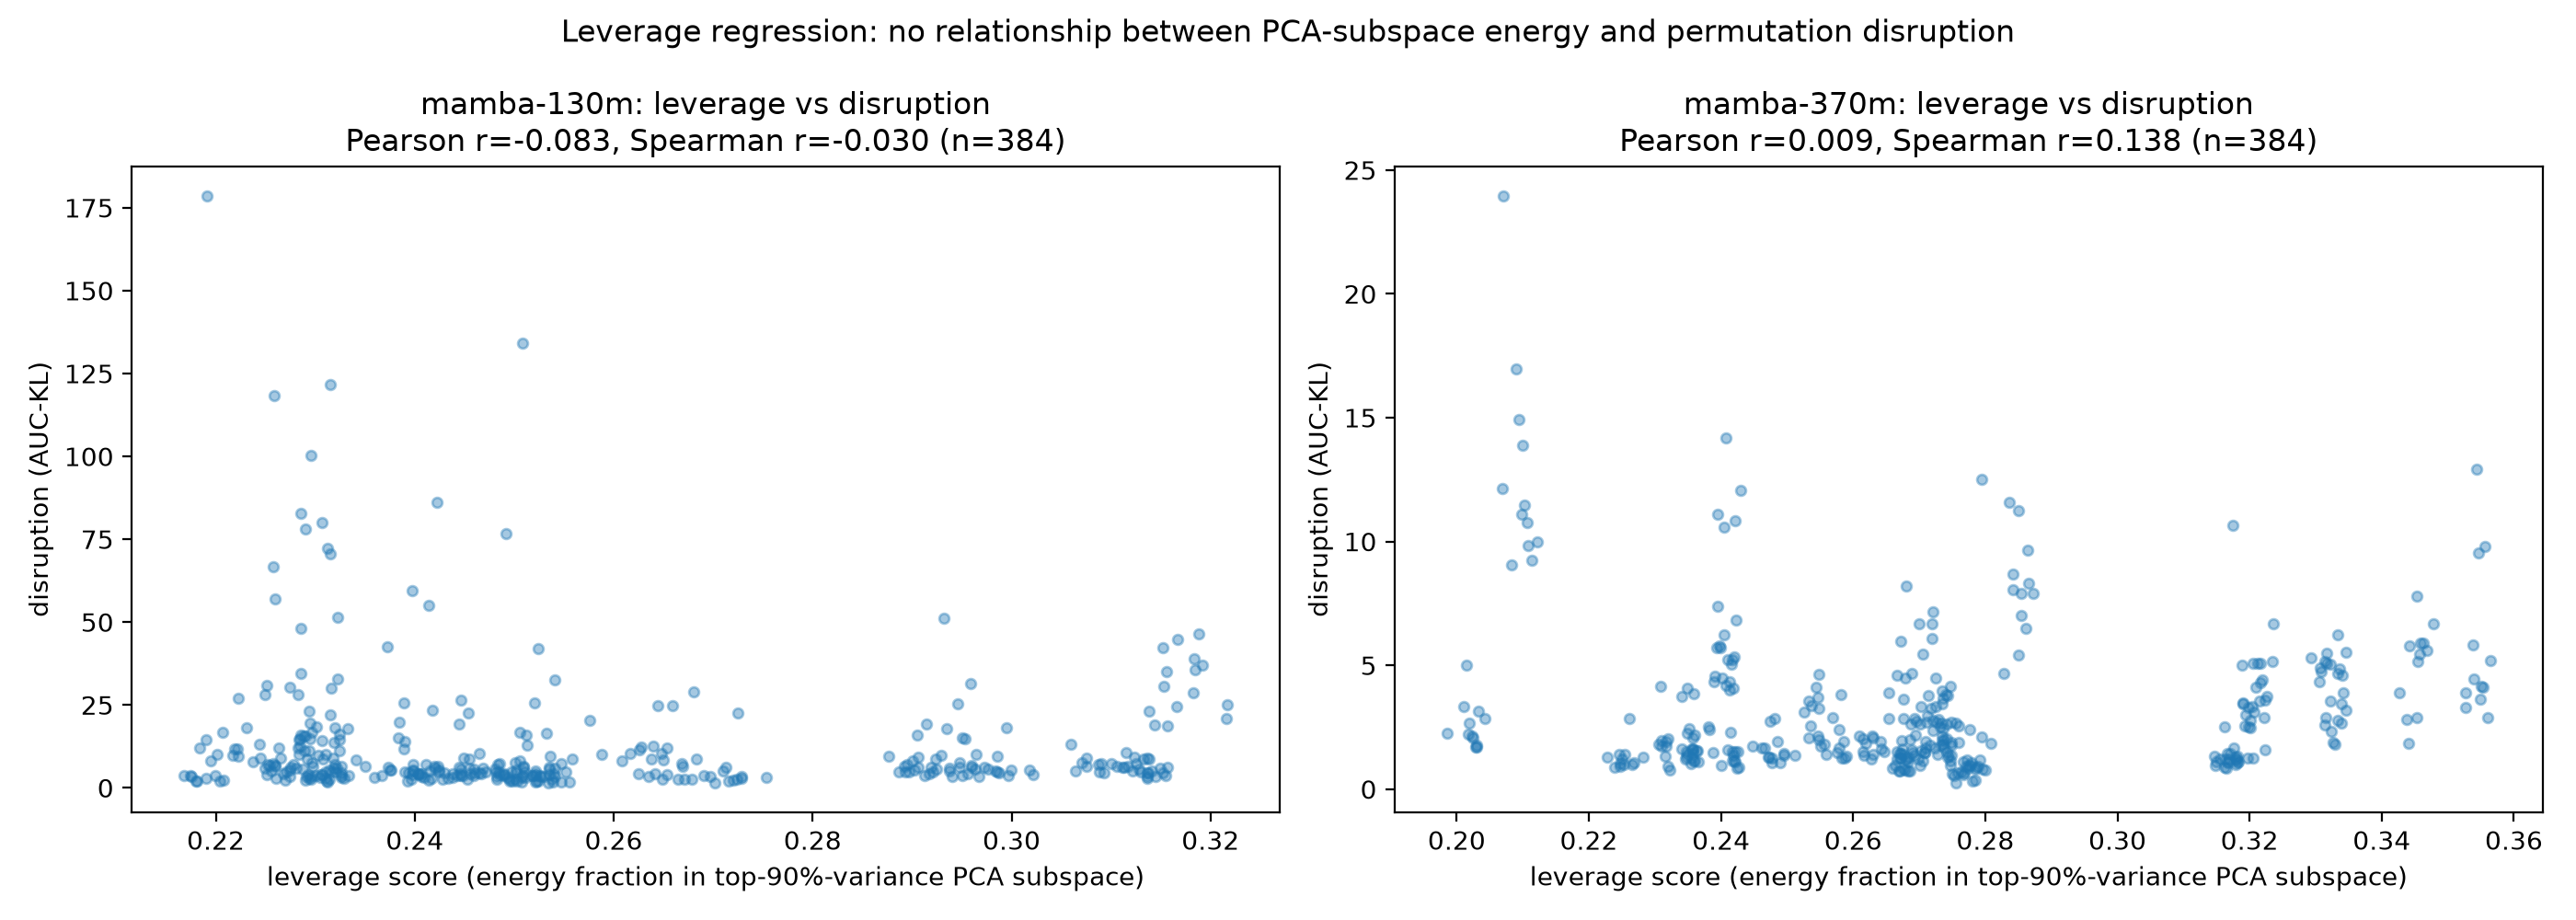
\includegraphics[width=0.9\textwidth]{figures/leverage_scatter.png}
  \caption{\todojay{Caption -- consider swapping for a dedicated participation-ratio-by-depth figure rather than the leverage scatter, which belongs in \S\ref{sec:critical-channel} instead.}}
\end{figure}

\subsection{Transplant ordering and the disruption law}
\label{sec:ordering}
\todojay{Monotonic ordering same $<$ related $<$ unrelated $<$ permuted,
Holm-Bonferroni corrected, $p<0.0004$ on all 6 links (3 links $\times$ 2
models). AUC-KL by condition:}
\begin{table}[h]
\centering
\begin{tabular}{lrr}
\toprule
Condition & Mamba-130M & Mamba-370M \\
\midrule
same-context     & \AucKlSameContextOneThreeM & \AucKlSameContextThreeSevenM \\
related-context  & \AucKlRelatedOneThreeM & \AucKlRelatedThreeSevenM \\
unrelated-context& \AucKlUnrelatedOneThreeM & \AucKlUnrelatedThreeSevenM \\
on-manifold noise& \AucKlOnManifoldOneThreeM & \AucKlOnManifoldThreeSevenM \\
Gaussian         & \AucKlGaussianOneThreeM & \AucKlGaussianThreeSevenM \\
permuted-real    & \AucKlPermutedOneThreeM & \AucKlPermutedThreeSevenM \\
\bottomrule
\end{tabular}
\caption{AUC-KL disruption by condition, seed 0, both models (paired, same pairs/baseline).}
\end{table}

\todojay{State the disruption law: $\mathrm{disruption} = k(1-\mathrm{similarity})$,
zero-intercept fit costs nothing vs.\ two-parameter OLS
(Pearson $r=$\PearsonROneThreeM/\PearsonRThreeSevenM, Spearman
$r=$\SpearmanROneThreeM/\SpearmanRThreeSevenM). This is the paper's
quantitative spine -- state it as such.}
\begin{figure}[h]
  \centering
  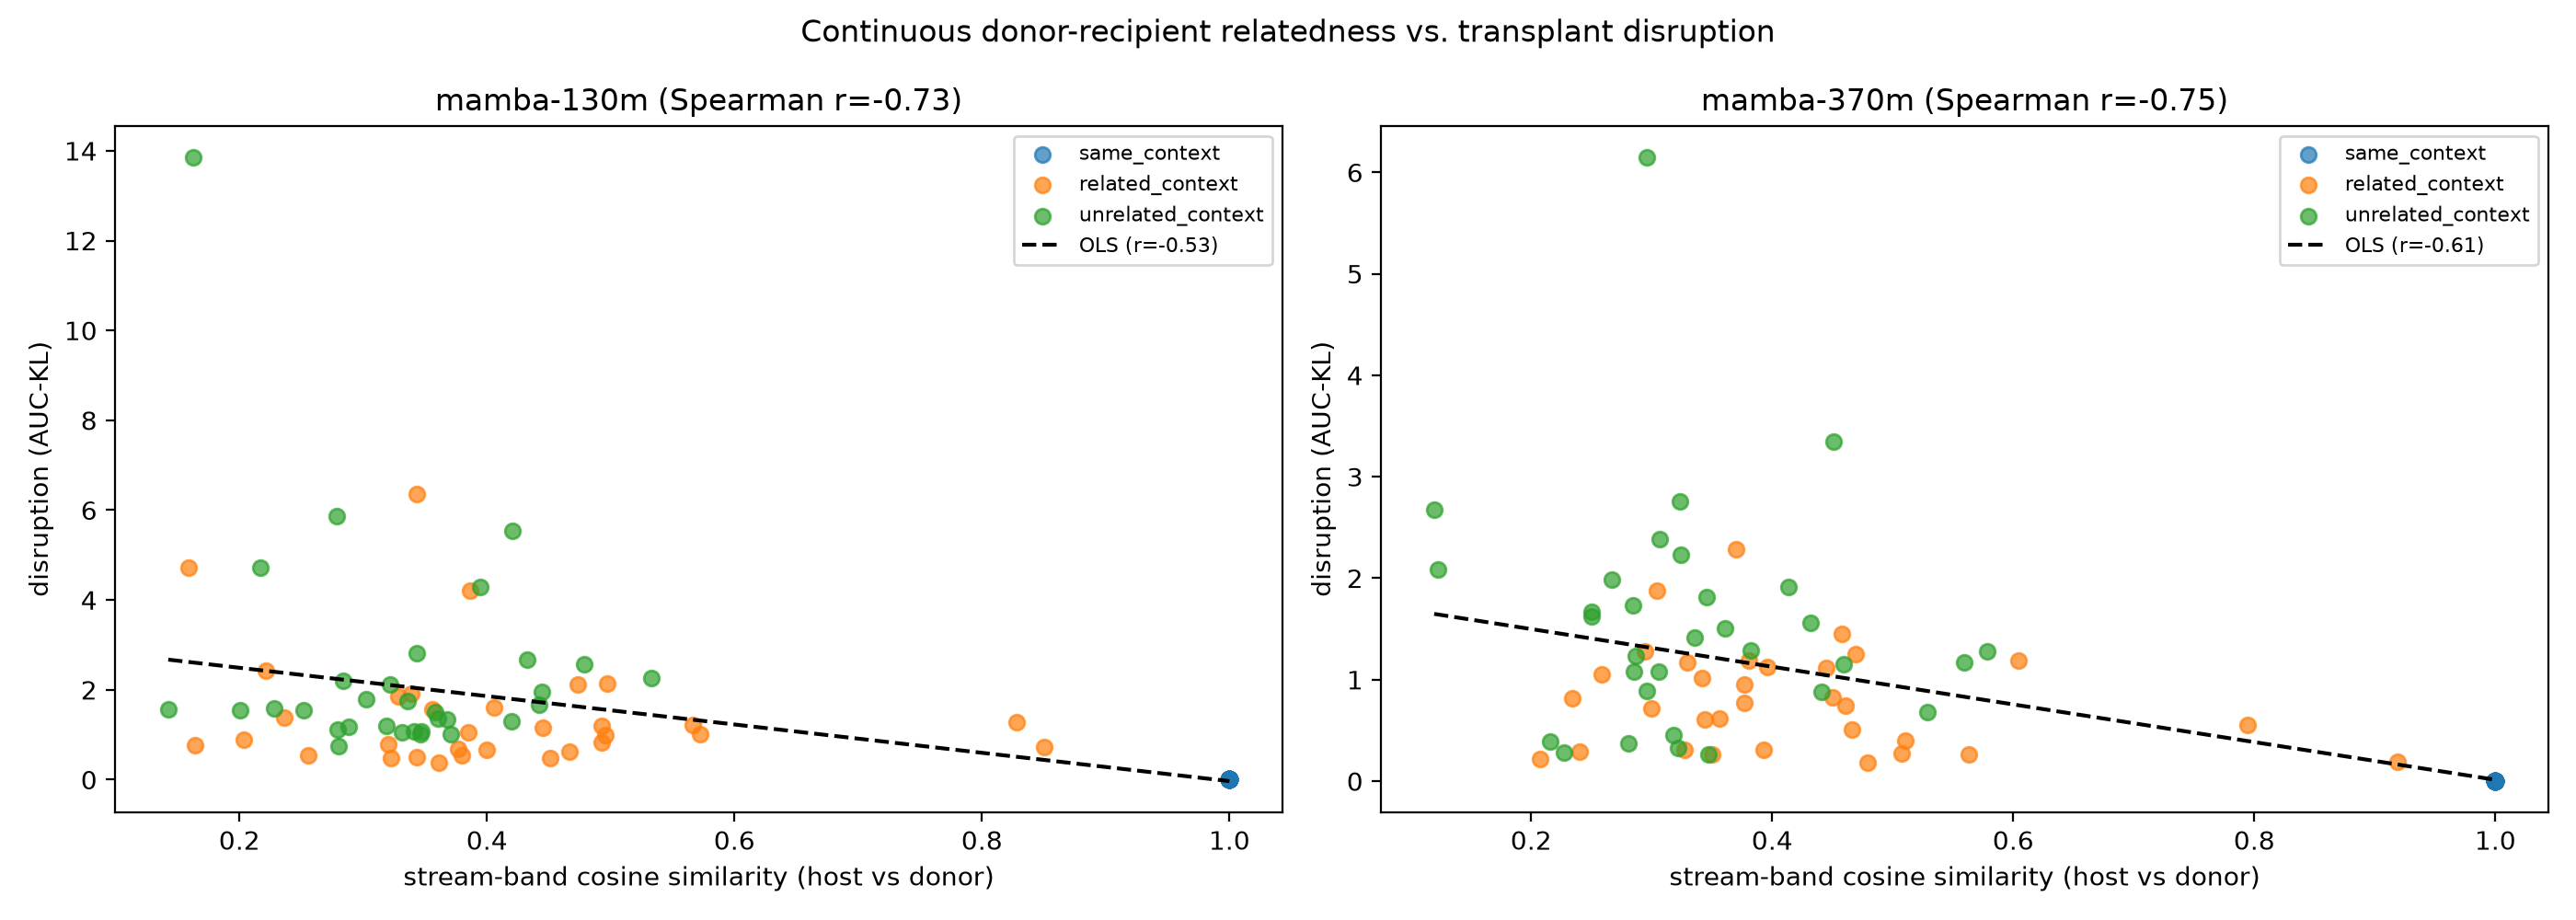
\includegraphics[width=0.9\textwidth]{figures/relatedness_plot.png}
  \caption{\todojay{Caption: continuous donor-recipient similarity vs.\ disruption, both models, with zero-intercept fit line.}}
\end{figure}

\subsection{Shape vs.\ content decomposition}
\label{sec:shape-content}
\todojay{Gaussian$\to$on-manifold gap (\GaussianMinusOnManifoldOneThreeM/\GaussianMinusOnManifoldThreeSevenM)
vs.\ on-manifold$\to$unrelated gap (\OnManifoldMinusUnrelatedOneThreeM/\OnManifoldMinusUnrelatedThreeSevenM):
shape accounts for \ShapeShareOneThreeM/\ShapeShareThreeSevenM\ of the
total gap, both models. State the convergence with \S\ref{sec:legibility}'s
correlational instrument -- two independent methods agreeing on
``mostly form, thinly content'' is the interpretive payoff.}
\begin{figure}[h]
  \centering
  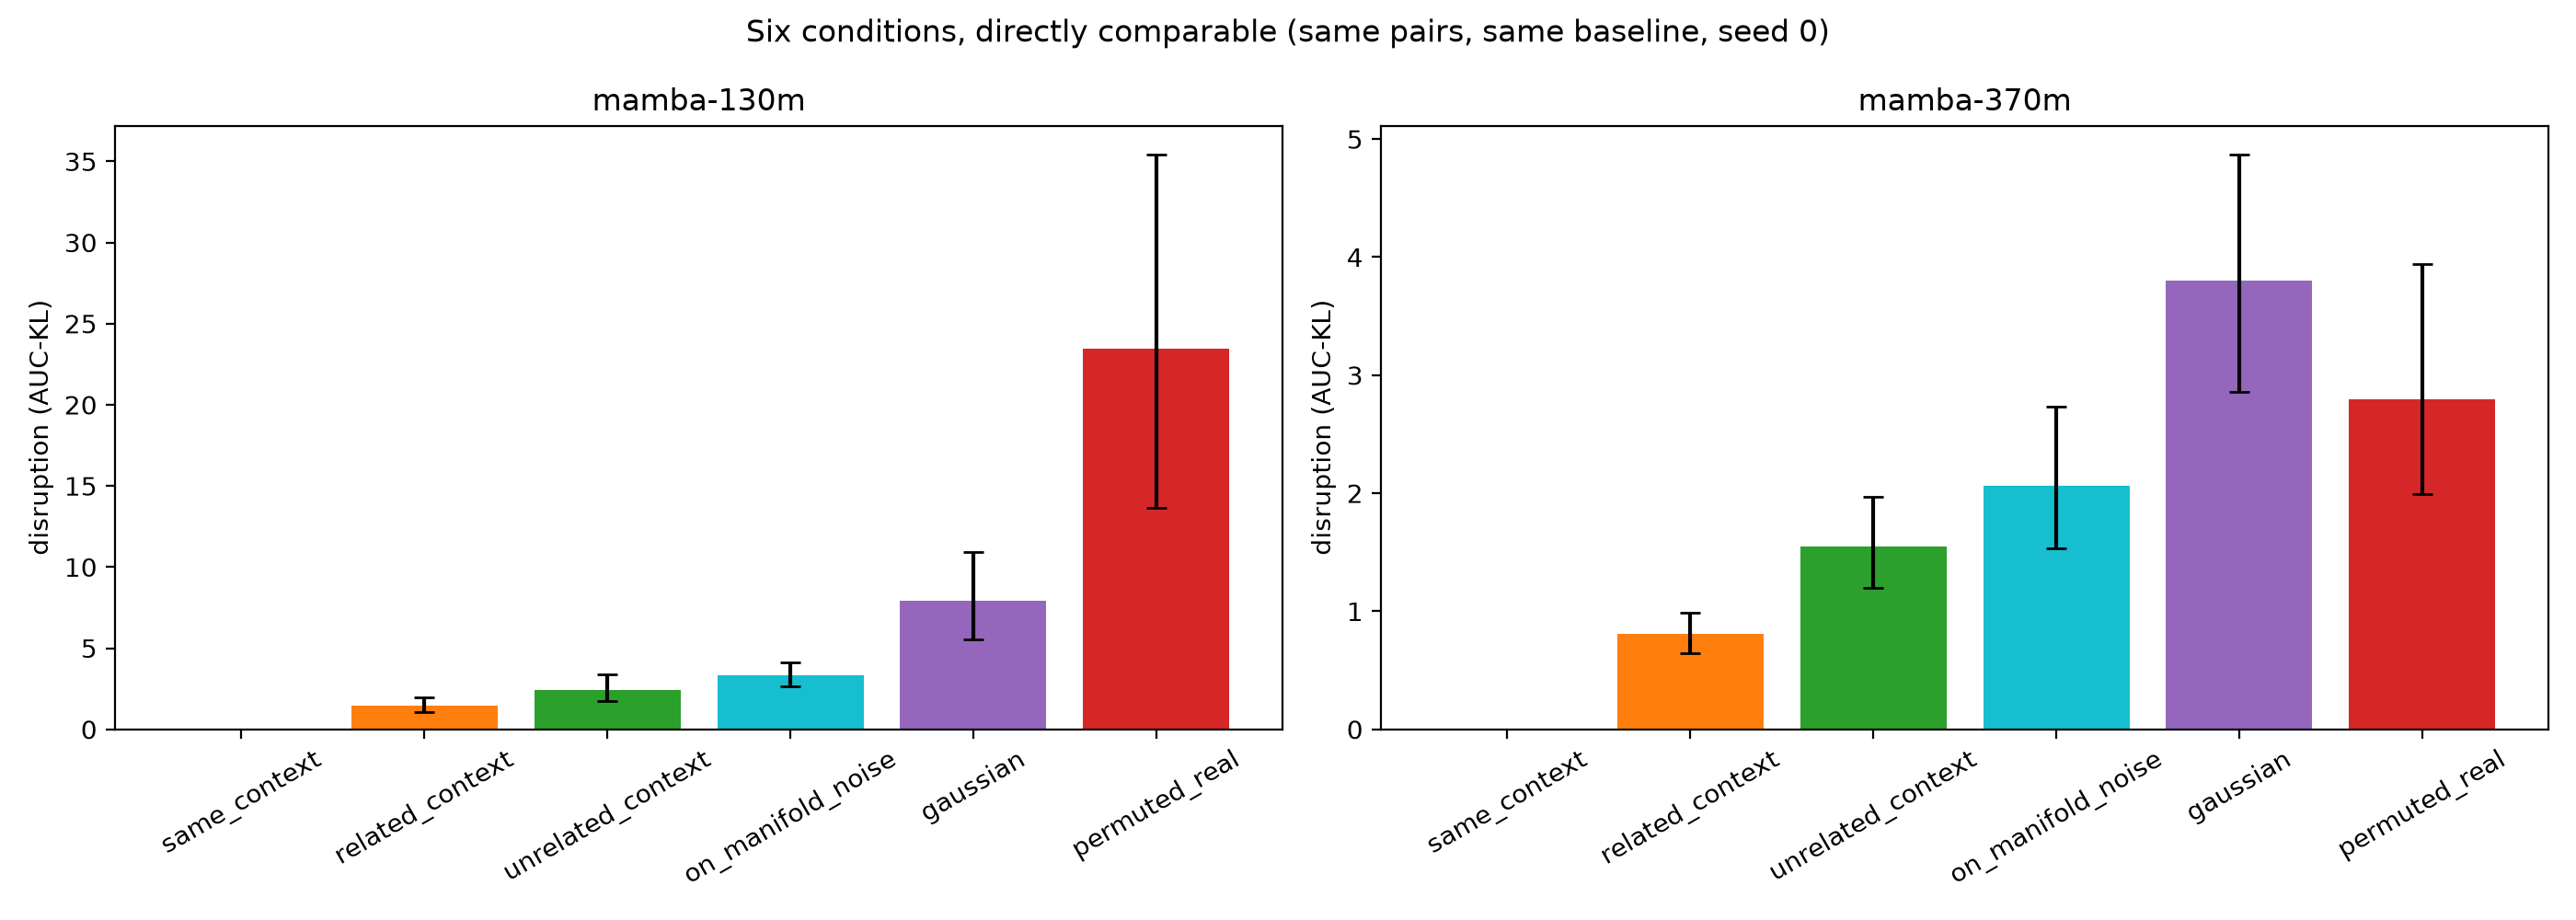
\includegraphics[width=0.9\textwidth]{figures/six_condition_bars.png}
  \caption{\todojay{Caption: all six conditions, paired, both models.}}
\end{figure}

\subsection{Critical-channel structure and the leverage null}
\label{sec:critical-channel}
\todojay{The 12-seed permutation distribution at Mamba-130M is
heavy-tailed/bimodal (most realizations track Gaussian's range, a
subset is 2--4$\times$ more disruptive). Broad PCA-subspace leverage
regression: null (Pearson $r=$\LeveragePearsonOneThreeM/\LeveragePearsonThreeSevenM).
Narrow critical-channel (top-PC1-3-loading coordinates) regression:
\emph{also} null, at every $k$ tested (3, 5, 10) -- report as a second
null, per \texttt{reports/phase1/critical\_channel\_check.md}. The
per-layer PC1 structural map (which raw coordinates dominate each
layer's top variance direction) stands as an independent descriptive
deliverable regardless of the null regression.}

\subsection{Provenance blindness}
\label{sec:provenance}
\todojay{Neutral characterization from \texttt{reports/phase1\_transplant\_triangulation.md}'s
``Provenance blindness'' section: the state accepts syntactically valid
foreign content far more readily than equal-magnitude noise, continuously
scaling with donor similarity; this is a characterization of the
undefended baseline, not a claim about exploitability or what any
deployed system does. Frame for AI-security relevance without
overclaiming.}

\section{Discussion}
\todojay{Full discussion -- Jay's voice. Suggested throughlines: (1) the
G1a/G1b dissociation as evidence stream and genuine state are different
kinds of object, not degrees of the same thing; (2) what ``mostly form,
thinly content'' implies for the interoceptive-loop design (protocol
\S6) -- the loop's ``leaning + certainty'' readout is exactly top-1-shaped,
matching the state's own native legibility shape (see Amendment 4's
margin note) -- lucky coincidence or the same architectural floor
showing up twice; (3) what remains open: P-A4-4's status, the
unexplained bimodal permutation distribution, whether the shape/content
ratio holds at larger scale (790M+, 3060-tier hardware).}

\subsection*{Gate G1}
Adjudicated 2026-07-08; full record \texttt{protocol/GATE\_G1\_DECISION.md}.

The transformer workspace's depth-localized organization does not port
to recurrent SSM state. The SSM organizes its readable signal
differently -- pervasive and early (\BandWidthPctOneThreeM\ /
\BandWidthPctThreeSevenM\ of depth in Mamba, peaking at layer
\PeakLayerOneThreeM\ of \NLayersFullAboveFloorOneThreeM's denominator,
the same absolute layer across a 2$\times$ depth difference) rather than
banded and mid-network (\BandWidthPctPyFourTen\ in Pythia-410M at
matched-ish scale) -- and its persistent state is a structured,
low-dimensional, causally-potent object that is not arranged the way
the workspace story predicted. P-A4-4's pre-registered localized-band
prediction failed decisively, in both models, in the direction against
the registrant.

This is a claim about the *representational* signature specifically
(lens-family readout) -- not that no workspace-like function exists in
SSMs at all. Whether a *functional*, causally-defined workspace exists
is a separate, harder, deliberately deferred question; representational
prominence and causal importance are known to come apart in SSMs, and
this project's own shape/content dissociation is one instance of that
gap. Scoped to the small tier (130M/370M) only.

\todojay{Downstream implications -- Jay's call, not resolved by the
gate decision itself: whether protocol \S4.4's hybrid-only pivot
(specified for a flat negative) applies to this non-binary outcome;
whether Phases 2-5 are superseded outright or need re-scoping around
what the state actually has (pervasive/early/thin) rather than what the
protocol assumed (localized/banded); what runs next.}

\section{Limitations}
\todojay{
\begin{itemize}
  \item Small-tier only (Mamba-130M/370M) on primary hardware; the
  protocol's confirmatory ladder ($\geq$790M) is unrun on this 4GB card
  -- an explicit, documented scope deviation (Amendment 1), not a claim
  the pattern holds at scale.
  \item Hardware deviation from the protocol's 12GB baseline (Amendment 1).
  \item Pile-10k substitute for the original Pile (host down); a
  shuffle-and-take draw per experiment, not a formally partitioned
  k-fold held-out scheme -- stated in \texttt{paper/reproducibility.md},
  not hidden.
  \item No custom CUDA kernels; HF's pure-PyTorch sequential-scan
  fallback throughout (slower, not wrong).
  \item $N=32$ pairs per transplant condition; single fixed snapshot
  position (token 16) per context for the state corpus and lens
  training, not sampled across positions within a document.
  \item State-corpus PCA's \texttt{dim\_99\%} figures approach the
  corpus's own $N=1{,}200$ at several layers (values near 1{,}000--1{,}100)
  -- likely underestimates, since SVD rank is capped near $N$;
  \texttt{dim\_90\%} (what Task 7's on-manifold condition actually uses)
  stays comfortably below $N$ everywhere and isn't subject to this caveat.
  \item Leverage and critical-channel regressions tested two
  operationalizations (broad PCA-subspace energy; narrow PC1--3-loading-ranked
  coordinate subsets at $k=3,5,10$), both null -- not an exhaustive
  search of possible mechanisms; the bimodal permutation-disruption
  pattern remains unexplained.
  \item Echo-partialling (\S\ref{sec:legibility}) rules out gross input-echo
  as the primary driver of the legibility floor but was tested with one
  echo definition (any-of-prefix and last-\NRecentK-tokens); a fuller
  three-way echo/output-prediction/neither tagging of lens top-$k$
  outputs, as protocol \S4.1 originally specified, was not attempted.
\end{itemize}
}

\section{Reproducibility}
See \texttt{paper/reproducibility.md} for exact commands, seeds,
checkpoint revisions, and the pre-registration/erratum trail.

\end{document}
